%!TEX root = ../thesis.tex

\chapter[Cooperative Multi-Robot Navigation]{Cooperative Multi-Robot Navigation --– SLAM, Visual Odometry and Semantic Segmentation}
\label{ch:cmrn}

\ifpdf
	\graphicspath{{Chapter4/Figs/Raster/}{Chapter4/Figs/PDF/}{Chapter4/Figs/}}
\else
	\graphicspath{{Chapter4/Figs/Vector/}{Chapter4/Figs/}}
\fi

This chapter describes three systems for multi-robot navigation: multi-robot SLAM for large environments, visual odometry for high odometric accuracy, and semantic segmentation for dynamic scene understanding.
Our multi-robot SLAM is capable of navigation, exploring and mapping a large-scale urban environments. Environmental exploration and mapping are achieved through wheel odometry and LiDAR, which interface through the Robot Operating System (ROS) framework on each robot. This system is distributed and decentralised whereby each robot performs localisation and mapping independently, while maintaining persistent maps are being transmitted to a ground control centre that verifies the map data.
Visual navigation in the form of visual odometry is used with minimal changes to the existing software and hardware framework. We use visual odometry as an alternative to wheel odometry, which is affected by wheel slip, a persistent error that accumulates over time.
Semantic segmentation complements object detection data from the LiDAR by introducing a pixel-based object recognition method that allows each robot and their visual odometry to vary its reaction based on the detected object class. These visual navigation subroutines can complement the existing mapping and localisation routines as an alternative solution.

\section{Introduction}
The University of Western Australia (UWA)'s multi-robot system (MRS)~\cite{boeing_wambot:_2012} comprises seven Pioneer 3AT-based outdoor robots. It was designed to solve the multi-robot simultaneous localisation and mapping (SLAM) problem through strongly coordinated behaviours with task allocations that are performed explicitly whereby each task is divided into subtasks that are dynamically allocated and re-allocated in response to changing conditions or failure~\cite{ortiz_task_2005}. In other words, this system is capable of structured communications while being aware of one another.

\nomenclature[z-mrs]{MRS}{Multi-robot system}
\nomenclature[z-uwa]{UWA}{University of Western Australia}

For an MRS to properly navigate an environment and perform cooperative tasks, these localisation estimates need to be robust. Our system uses a contained localisation system to allow for rapid deployments in unstructured/mixed indoor/outdoor environments, which is originally presented in~\cite{reid_large-scale_2016}. Path planning and obstacle avoidance currently follow our implementation in~\cite{a._boeing_real-time_2012, a._boeing_cooperative_2011}. We use a multi-robot SLAM (MR-SLAM) solution to localise robots through the construction of a shared local map. The MR-SLAM problem is complex, whereby localisation is achieved through the registration of each robot in a consistent, global coordinate system, in which large amounts of sensor data fusion must occur on-line. Additionally, these robots often rely on wireless communication that is often lossy and subject to interferences with variations in latencies and bandwidth. Loop closures that are predominant in SLAM problems become more challenging, as they create large sequences of constraint cycles, which can cause a combinatorial increase in computational complexity. This problem stems from the variations between the robots' vantage points where uncertainties in data association might arise due to the pairings between object detections and sensor measurements.

\nomenclature[z-mrslam]{MR-SLAM}{Multi-robot simultaneous localisation and mapping}

MRS projects presented in the recent literature~\cite{luft_recursive_2018, garzon_multirobot_2016, best_dec-mcts:_2018} demonstrated a combination of low-level capabilities such as cooperative SLAM, exploration, object identification, object tracking, and object manipulation. A comprehensive review is available in~\cite{saeedi_multiple-robot_2016, abdulgalil_multi-robot_2019}. These systems are off-line or on-line. Off-line systems collect the first sensor data that is processed at a later stage, while on-line systems perform MR-SLAM and other tasks in real time during deployment. It is worth noting that off-line systems are typically deployed based on their ease of implementation and prototyping, while often relaxing limitations imposed on computation and communication requirements. Additionally, many works are often implemented in constrained environments, such as in indoor laboratories~\cite{jung_development_2015, koch_multi-robot_2016}, thereby preventing the robots from exposure to environmental irregularities, including noise, temperature, illumination, and seasonal variations. These systems can therefore be cheaper and more convenient to implement, as they usually do not require long-range mobility and sensors. Conversely, our MRS was designed for deployment in unconstrained, outdoor urban environments, requiring higher performance sensors and more rugged robots.

The incorporation of visual navigation onto the MRS stems from our motivation to solve problems relating to wheel slip in odometry and scene understanding. Works that implement visual odometry in robots~\cite{kunii_mobile_2017, sun_sequentially_2017, kim_effective_2016} have proven that its ability to reduce the accumulating error caused by wheel slip can lead to more robust SLAM solutions. Visual SLAM algorithms such as ORB-SLAM~\cite{mur-artal_orb-slam2:_2017} and LSD-SLAM~\cite{engel_lsd-slam:_2014} are often implemented on robots, with favourable outcomes. Likewise, scene understanding can be applied alongside obstacle detection from LiDAR measurements, such as classifying static and dynamic obstacles~\cite{zhou_dynamic_2018}. For our application, we have decided to apply semantic segmentation for scene understanding, as it offers a pixel-wise classification of a captured scene while being versatile and compatible with low-cost camera setups.

\section{Robot Hardware Design}
\begin{figure}[H]
	\centering
	\includegraphics[width=\linewidth]{fig1}
	\caption[MRS UGV with hardware modules]{Photo illustrating an single MRS UGV with its hardware modules as labelled.}
	\label{fig:4:design}
\end{figure} 

Each unmanned ground vehicle (UGV) in our MRS is fitted on top of a Pioneer AT3~\cite{adept_technology_inc._pioneer_nodate} base, which provides a chassis, differential drive wheels with motor controllers and encoders, and batteries (see Fig.~\ref{fig:4:design}). High-level controls are performed through an Intel Core 2 Duo automotive PC that is connected to several sensors (see Figure~\ref{fig:4:design}). The sensors comprise an ibeo LUX 4 LiDAR~\cite{autonomoustuff_ibeo_nodate}, a SICK LMS-111 LiDAR~\cite{sick_ag_lms111-10100_nodate}, a Hokuyo URG-04LX LiDAR~\cite{hokuyo_automatic_co._ltd._scanning_nodate}, an Xsens MTi inertial measurement unit (IMU)~\cite{xsens_mti_nodate}, a QStarz GPS receiver~\cite{qstarz_international_co._ltd._bt-q818xt_nodate}, wheel odometry on the Pioneer base, and a Logitech Sphere PZT camera~\cite{logitech_quickcam_nodate}. Communications are performed between UGVs and base station through a Ubiquity Pico Station 2HP~\cite{ubiquiti_networks_picostation2hp_nodate} over a Wi-Fi mesh, with an RF Innovations 900 MHz radio~\cite{sti_engineering_pty_ltd_rfinnovations_nodate} as a redundant communications link. The Pico Station, LUX 4, and LMS-111 interface via 100 Mbps Ethernet, while the other sensors interface through USB 2.0.

\nomenclature[z-ugv]{UGV}{Unmanned ground vehicle}

The sensors perform LiDAR-based SLAM, whereby the LiDAR array maps the environment horizontally and has a 20 m, \ang{270} range at 25 Hz; the URG-04LX is mounted vertically and has a 4 m, \ang{240} range at 10 Hz; and the LUX 4 is mounted horizontally and has a 50 m, \ang{110} range that spans across four parallel, horizontal layers. The LMS-111 is used as the main SLAM sensor, where is it placed 0.5 m above ground to scan a single-layer horizontal plane. This results in 1080 measurements that translate to 2D ``slices'' of the environment around a 20 m radius. The other LiDARs mounted on the UGV are used for object/obstacle detection and tracking.

\section{Cooperative Localisation and Navigation}\label{sec:4:cln}
We incorporate our hybrid-decentralised and distributed MR-SLAM system onto the UGVs, which allows the decentralised UGVs to build distributed global grid-maps and navigate large urban areas~\cite{r._reid_large-scale_2011, r._reid_cooperative_2013}. Using this system enables the system to be deployed rapidly while allowing SLAM on the UGVs with minimal reliance on a ground control system (GCS).

\nomenclature[z-gcs]{GCS}{Ground control system}

\subsection{Mapping}

\begin{figure}[H]
	\centering
	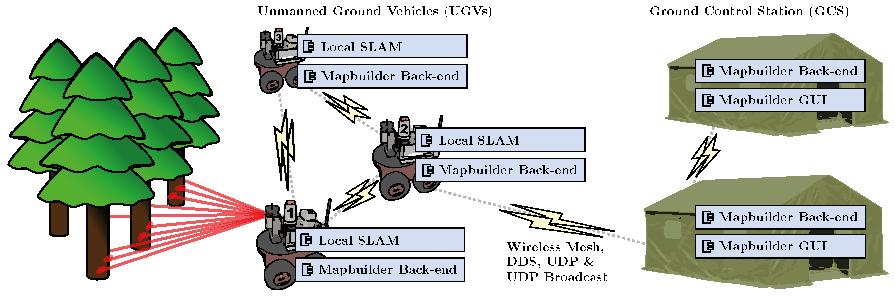
\includegraphics[width=\linewidth]{fig2}
	\caption[MR-SLAM architecture and software development diagram]{The MR-SLAM architecture and software development diagram showing the software components run on the GCS and UGVs.}
	\label{fig:4:mrslam}
\end{figure} 

A typical deployment scenario of the MR-SLAM system is illustrated in Fig.~\ref{fig:4:mrslam}, showing that the back-end is executed across UGVs and GCSs. Each back-end instance stores a local copy of all submaps and constraints, which are then optimised and fused, building global maps; new loop closure constraints between submaps are also searched. Submaps are rectangular grid-maps with dynamically increasing dimensions determined by the LiDAR's maximum range $R$, the environment's shape, and a threshold heuristic described later in this section.

Local SLAM is performed independently on each UGV whereby a single-robot SLAM algorithm builds its own submap by processing its sensor data, which is then broadcasted across the mesh network. Graphical user interfaces (GUIs) are installed on GCS computers to enable operators to view and manipulate global and submaps and interact with pose graphs through a point-and-click interface.

\nomenclature[z-gui]{GUI}{Graphical user interface}

A global grid-map is fused through several overlapping submaps that are obtained from the SLAM algorithms running on each UGV, thereby achieving a distributed map-building sequence. The fusion algorithm searches for overlaps in the grid-maps and subsequently determines if the cells in the global grid-map are occupied, free, or unknown. Each submap initialises with a local coordinate frame on the global frame with its submap pose $p^W_a$, which is estimated through pose graph optimisation in a global Euclidean coordinate frame $W$. Given the UGV pose $r^a_t$ always broadcast relative to $p_a^W$, and that each submap is created with the UGV at its origin, therefore $r^a_0 = [0, 0, 0]^\intercal$, and the UGV's time-varying pose in the global frame is thus:
\begin{align}
r^W_t = p^W_a \oplus r^a_t
\end{align}
Each submap is assigned a 128-bit hexadecimal universally unique identifier (UUID) and exists either in an ``open'' or “closed” state, where they are always created through an “open” state to indicate that an occupied UGV is in the process of building it. Once map building is complete, the submap changes to a “closed” state to render the area immutable and non-traversable by any UGV, only allowing the back-end to update its pose, thereby fusing it onto the global grid-map. Having these states increases the robustness of the MR-SLAM system while ensuring its logic simplicity. A UGV can only occupy a single submap at any given time, and these “open” submaps are often connected to an adjoining “closed” submap. At the creation of a new submap, its map and pose uncertainty is reset. Using this approach enables the system to minimise bandwidth, storage, and redundancy across the MR-SLAM back-end.

\nomenclature[z-uuid]{UUID}{Universally unique identifier}
\nomenclature[a-rab]{$r_a^b$}{UGV pose}  
\nomenclature[a-pab]{$p_a^b$}{Submap pose}  
\nomenclature[r-w]{$W$}{Euclidean coordinate frame}
\nomenclature[s-t]{$t$}{Time}  

Using a ray tracing technique based on~\cite{bresenham_algorithm_1965}, the LiDAR scans obtained while navigating a submap is aligned and fused into a single 2D occupancy grid-map, which maintains an accurate representation of the environment. The LiDAR scans are aligned with scan matching prior to ray tracing to circumvent the accumulation of minor quantisation noise, which is done through a batch rounding of these LiDAR measurements to the nearest grid cell using the grid-map representation.

Aside from quantisation noises, UGV pose uncertainties are also prevalent while it is building a submap. Although a UGV always initialises a new submap with no pose uncertainties, this uncertainty will always accumulate whenever the UGV is manoeuvring, with odometric noise as its main contributor. Therefore, it is more pronounced in larger areas. To solve this problem, the algorithm initialises a new submap whenever this uncertainly surpasses a set threshold, which is determined by comparing the current angular pose uncertainty against the average distance to obstacles in the environment, estimating the amount of “blurring” in distant grid-map cells. Current LiDAR scans will not be fused if a new submap is triggered using this approach; using this heuristic thus minimises distortions entering the submap grid-map, and large distortions that result in misaligned LiDAR scans can be prevented. The algorithm then transfers this accumulated uncertainty's covariance into the new constraint's covariance that is used to connect the old and new submaps through a maximum likelihood estimation.

By assuming an average distance between submaps $D$, the maximum overlap between a sequence of submaps separated by $D$ is given by a ratio:
\begin{align}
\text{Maximum overlap} = \frac{2R}{2R + D}
\end{align}
The MRS yields a maximum submap overlap of 93\%, which implies that the same UGV could create submaps that overlap the same area up to 15 times. This overlapping redundancy is required to allow the distributed back-ends to compare and align map data.

\nomenclature[a-D]{$D$}{Ground distance}  

\subsection{MR-SLAM Architecture}
With reference to Fig.~\ref{fig:4:mrslam}, we have identified the functional roles of the software components as Table~\ref{tbl4:fr}, which illustrates a minimalistic logical design diagram that considers a single UGV and GCS.

\begin{table}[H]
	\caption{Functional requirements of software components}
	\centering
	\label{tbl4:fr}
	\begin{tabularx}{\textwidth}{ p{2cm} X  X X }
		\toprule
		Component        & Input                                                                      & Behaviour                                              & Output                                                                     \\ \midrule
		Local SLAM       & Sensor data (LiDAR, odometry, IMU, GPS)                                    & Performs local SLAM, creates a sequence of submaps     & Broadcasts submap data, constraints, real-time UGV pose estimates          \\
		MR-SLAM back-end & Submap data from all UGVs, submap constraints, ground-truth constraints    & Optimises pose graphs, fuses submap data, searches for & Global or windowed maps, submap pose estimates, submap constraints         \\
		MR-SLAM GUI      & All MR-SLAM messages, GUI events; for example, keystrokes and mouse clicks & Displays global maps, interprets operator commands     & Messages that alter graph structure; for example, ground-truth constraints \\ \bottomrule
	\end{tabularx}
\end{table}

The class diagram in Fig.~\ref{fig:4:cd} illustrates the various message types used by the system for MR-SLAM, which are all derived from the Submap message class. All messages are time-stamped with the source participant's priority and the submap UUID.

\begin{figure}[H]
	\centering
	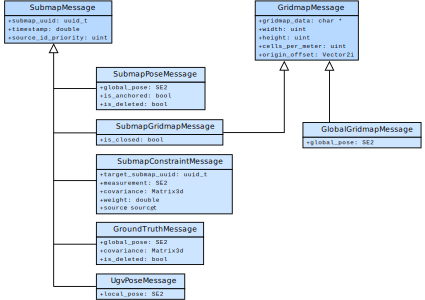
\includegraphics[width=0.9\linewidth]{fig3}
	\caption[MR-SLAM class diagram]{A class diagram showing the MR-SLAM system’s message types and their variables.}
	\label{fig:4:cd}
\end{figure}

For the local SLAM front-end, we use a heuristic-driven EKF-SLAM~\cite{dissanayake_solution_2001} single-robot algorithm that takes all sensor data and outputs submaps, constraints, and real-time pose estimates, which are broadcasted over the mesh network. We have designed this front-end based on the following requirements:
\begin{itemize}
	\item To estimate UGV pose and broadcast in real-time at more than 10 Hz locally, or 1 Hz globally.
	\item To build 10 cm submap grid-maps that are broadcasted at more than 1 Hz locally, or 0.2 Hz globally.
	\item To robustly handle moving objects including human gaits up to 6 km/h.
	\item To handle challenging sensing conditions such as sparse and/or featureless areas.
	\item To detect odometric errors to minimise submap corruption.
	\item To compress submap grid-maps before broadcasting.
	\item To use less than 25\% of total computation and memory footprint.
\end{itemize}
Likewise, the back-end requirements of our MRS are:
\begin{itemize}
	\item To optimise pose graphs robustly and efficiently at less than 5 seconds per iteration.
	\item To output large ($5000\times5000$) grid-maps to the local partition at more than 1 Hz.
	\item To match submaps to generate robust constraints at less than 5 seconds per match.
	\item To broadcast \textbf{SubmapPose} messages globally to maintain decentralised pose graph.
	\item To output \textbf{SubmapPose} updates to the local partition at more than 1 Hz.
\end{itemize}

\subsection{SLAM Implementation}
We apply EKF-SLAM with scan matching which builds submaps by aggregating LiDAR scans at every 20 cm of movement or \ang{20} of rotation, where pose estimation is achieved through an EKF. Scan matching was incorporated to reduce computation requirements by using the described threshold heuristics to decide when a current submap should be closed, which is augmented by a threshold on the percentage of LiDAR returns that are aligned successfully. This method enables the detection of matching failures, especially in sparse environments. EKF is used to estimate the UGV’s pose by initiating each cycle to predict its current pose using the latest wheel odometry and IMU data, which aligns the LiDAR scan against the current submap through scan matching~\cite{censi_accurate_2007}. RANSAC~\cite{martin_a._fischler_random_1981} is also incorporated to reject outliers in the form of moving objects. The EKF and pose estimate is subsequently updated using this scan matching alignment method. Odometric noises that are present in the EKF update are adjusted according to the local ground slope gathered from the pitch and roll measurements from the IMU. An increase in slope leads the module to assume an increase in odometric noise due to wheel slip, thereby switching the filter preference for scan matching over odometry.

\begin{figure}[H]
	\centering
	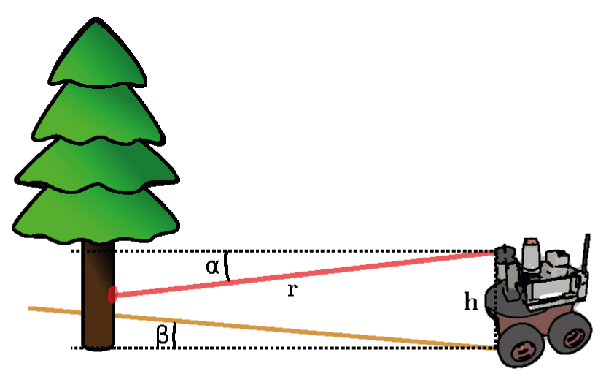
\includegraphics[width=0.6\linewidth]{fig4}
	\caption{Lengths and angles used for calculating the local SLAM prefilter.}
	\label{fig:4:slampf}
\end{figure}

To filter these errors using the IMU, we assume that (1) the terrain inclination is less than $\beta_\mathrm{max}$, and (2) the terrain follows the “Manhattan World”~\cite{coughlan_manhattan_2003} assumption. With reference to Fig.~\ref{fig:4:slampf}, each LiDAR measurement range $r$ is first corrected to account for the declination $\alpha$ from the same measurement as $r\cos\alpha$, whereby an inequality is obtained referencing the height of the LiDAR mounted above the ground $h$.
\begin{align}\label{eqn4:4}
0 < h - r\sin\alpha - r\cos\alpha \cdot \tan\beta_\mathrm{max}
\end{align}
To prevent any measurements from grazing the ground, any instance of $r$ with declination $\alpha$ that dissatisfies \eqref{eqn4:4} is filtered. LiDAR measurements that are corrected and filtered will then be passed to the SLAM algorithm.

\nomenclature[g-a]{$\alpha$}{Declination}    
\nomenclature[g-a]{$\beta$}{Inclination}    
\nomenclature[a-h]{$h$}{Height}  
\nomenclature[a-r]{$r$}{Measurement range [Chapter~\ref{ch:cmrn}]}  


\subsection{UGV/GCS Communications}
Communications between UGVs and GCSs are facilitated through a Wi-Fi mesh network over the IEEE 802.11n standard in a multi-hop configuration over a data distribution system (DDS), which provides a publisher-subscriber framework that provides robust real-time communications. Publishers are separated into partitions which are either global (all participants) or local (within a participant). Global partitions are mostly used to prevent network overloads, as the local partition is used for high-rate inter-process communications, where messages are passed over a shared memory between the front-end, back-end, and other high-level MRS software components.

Messages are broadcasted by the front-end as submaps are closing in the form of compressed grid-map data and the constraint that links the closed submap to the new one. Incomplete grid-maps for open submaps are also broadcasted to visualise real-time global maps; these maps are flagged to indicate that they are not yet immutable. The front-end broadcasts three distinct, time-stamped message types with a fixed DDS buffer size n with varying quality of service (QoS) priorities:
\begin{enumerate}
	\item \textbf{SubmapConstraint} ($n = 1000$) defines the entire pose graph structure. A large buffer size is allocated for the series of small yet vital messages.
	\item \textbf{SubmapGridmap} encodes the actual shape of the environment, constituting most of the MR-SLAM data, which are either open or closed.
	\begin{enumerate}
		\item \textbf{Open} ($n = 0$) grid-maps are disposable as they are periodically broadcasted by the front-end, these are sent to the local partition at the LiDAR’s scan rate.
		\item \textbf{Closed} ($n = 100$) grid-maps have higher priority as they are only transmitted once.
	\end{enumerate}
	\item \textbf{UGVPose} ($n = 0$) are broadcasted frequently in real-time, which stales quickly and is subsequently disposable. These are also sent to the local partition at the LiDAR’s scan rate.
\end{enumerate}
A rendering algorithm ray traces the accumulated LiDAR scans into an empty grid map based on the methods described in~\cite{bresenham_algorithm_1965}. The grid-map data is segregated into $32\times32$ cell tiles that are broadcasted over UDP on a $50:1$ compression ratio.

\nomenclature[z-dds]{DDS}{Data distribution system}
\nomenclature[z-qos]{QoS}{Quality of service}

Likewise, the back-end’s publishing policies are:
\begin{enumerate}
	\item \textbf{SubmapPose}:
	\begin{enumerate}
		\item \textbf{Global Partition} ($n = 0$) does not require delivery guarantees since priority-based filters synchronises this between participants.
		\item \textbf{Local Partition} ($n = 0$) does not require QoS as DDS uses shared memory to delivery real-time submap pose estimates.
	\end{enumerate}
	\item \textbf{SubmapConstraint} ($n = 1000$) is assigned with the highest priority as they define the entire pose graph structure, hence a large buffer size is allocated.
	\item \textbf{GlobalGridmap} ($n = 0$) are delivered through shared memory by DDS in real-time; QoS is therefore not required.
\end{enumerate}

\subsection{Loop Closures}
A loop closure is an event that occurs when a UGV revisits a location it has previously threaded, thereby correcting its accumulated errors. The identification of loop closures occurs between overlapping submap pairs and spatially similar grid maps, which are broadcasted as new constraints that form cycles in the distributed pose graphs, bearing residual errors that require optimisation. The back-end searches for local loop closures between “open” submaps in real-time, especially when multiple UGVs are operating overlapping areas to ensure proper localisation and prevent the accumulation of errors. Using this method enables our system to efficiently accommodate high rates of loop closures and map changes in real-time.

The large number of loop closures generated by the system, as well as the distributed algorithm design, prompted us to utilise the graphics processing unit (GPU) to search for loop closures and merge submaps. Additionally, descriptive spatial relationships between submaps are extracted using a grid-map correlation algorithm on the GPU that calculates likelihood volumes and extracts multimodal Gaussian constraints. Using robust multimodal constraints enables the algorithm to preemptively add loop closures to the pose graph and perform outlier rejection by consensus.

\begin{figure}[H]
	\centering
	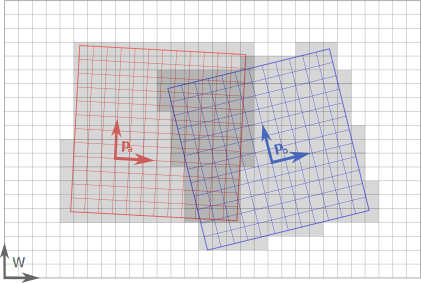
\includegraphics[width=0.7\linewidth]{fig5}
	\caption[Occupancy grid-map fusion]{Occupancy grid-map fusion illustrating two submap grid-maps with their origins $p^W_a$ and $p^W_b$ to be fused onto the global output grid-map $W$ shown as grey grids.}
	\label{fig:4:ogm}
\end{figure}

An overlapping submap pair also initiates an occupancy grid-map fusion algorithm. To achieve the fusion described in Fig.~\ref{fig:4:ogm}, we use a GPU-based approach whereby the algorithm checks for each overlapping cell in the output grid-map and performs a transformation of that cell in its 2D coordinates into the submap’s coordinate frame, subsequently fusing it into the output cell based on the corresponding submap cell value.

To optimise complex multimodal Gaussian constraints, we utilised a continuous mode blending optimisation technique that is based on non-linear least-square approaches and exhibits convergence properties that are representative of the underlying multimodal constraint distributions.

\subsection{SLAM Evaluation}
For the evaluations described here, ten UGVs were deployed to explore an $80\times40$ m environment. The total elapsed time was 36 minutes~\cite{reid_large-scale_2016}. The SLAM routine was completed with minimal user intervention whereby the UGVs autonomously explore the environment while displaying their progress in real-time onto the MR-SLAM system’s GUI. This process follows our approach in~\cite{s._lopes_autonomous_2011} and is illustrated in series across Figs.~\ref{fig:4:slamstart} through~\ref{fig:4:slamend} with timestamps on the upper right corner of the images in minutes and seconds; the total odometry across all UGVs is presented in meters at the lower right corner; UGVs are shown as dots with colour-matched lines showing their trajectories; pose graphs are green with dots, lines, and red triangles representing submap poses, submap constraints, and ground truth constraints, respectively.

The UGVs start at the southeast corner of the warehouse (see Fig.~\ref{fig:4:slamstart}), where two teams split to explore the west and north sections, respectively. Both teams explore independently until a loop closure is evident, as illustrated in Fig.~\ref{fig:4:slammmid}, where the first team is about to exit via the southwestern corner. The exploration forms a total closed path length of 230 m that is measured after the separation of the UGVs in the first room. The final result is presented in Fig.~\ref{fig:4:slamend}. This corresponds to about 70 constraints in the pose graph. Based on 88 samples collected across the surveyed area, the root-mean-square (RMS) error was calculated to be $\approx0.27$ m.

\nomenclature[z-rms]{RMS}{Root-mean-square}

The 2D correlation between each submap in Fig.~\ref{fig:4:mmc} is represented by each slice, with a $\pm3$ m translation variation along with $x$ and $y$-axes at a fixed angular rotation. For example, the middle row represents rotations of $-6$°, $-3$°, 0°, 3°, and 6°, respectively. The 2D ellipses represent three-sigma covariance modes through a Gaussian mixture model that fits the maximum likelihood volume. Occlusions have reduced the overlapping area of occupied cells (black) between the submap pair, and the matcher’s output is mostly dominated by an array of columns in the environment.

\begin{figure}[H]
	\centering
	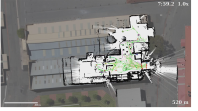
\includegraphics[width=0.8\linewidth]{fig7}
	\caption[SLAM output (starting)]{SLAM output showing the UGVs starting at the southeastern corner of the environment.}
	\label{fig:4:slamstart}
\end{figure}

\begin{figure}[H]
	\centering
	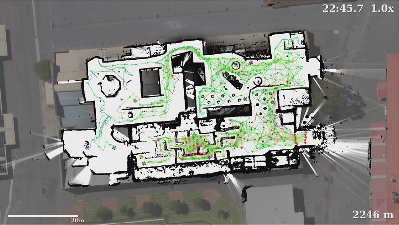
\includegraphics[width=0.8\linewidth]{fig6}
	\caption[SLAM output (loop closure)]{SLAM output showing loop closure between both teams, with the first team about to exit via the southwestern corner.}
	\label{fig:4:slammmid}
\end{figure}

\begin{figure}[H]
	\centering
	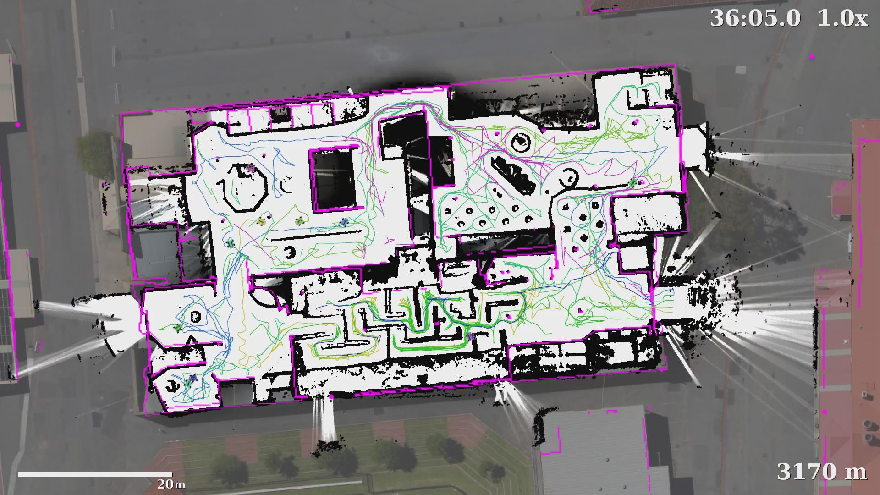
\includegraphics[width=0.8\linewidth]{fig8}
	\caption[Completed global grid-map]{Completed global grid-map with ground truth overlaid in magenta.}
	\label{fig:4:slamend}
\end{figure}

\begin{figure}[H]
	\centering
	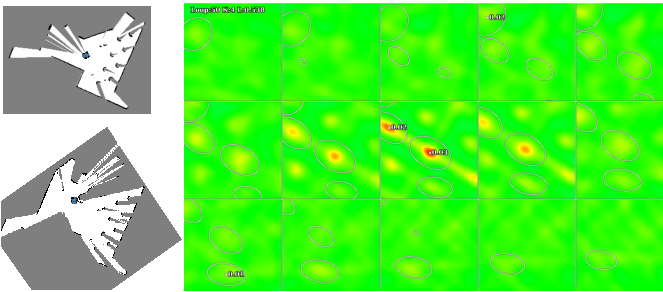
\includegraphics[width=\linewidth]{fig9}
	\caption[Multimodal constraint output]{Example of multimodal constraint output with perceptual aliasing. The correlation results for a test area with perceptual aliasing that was caused by repetitive geometry. It shows an overlapping submap pair (left) along with 15 slices through their constraint likelihood volume.}
	\label{fig:4:mmc}
\end{figure}

\section{Visual Odometry}\label{sec:4:vo}
While some effort was made to circumvent wheel slip accumulation in Section~\ref{sec:4:cln}, other works have demonstrated that visual odometry is often an effective solution to this problem~\cite{aqel_review_2016}. In the case of the MRS, this can be incorporated with no hardware or sensor modifications. Taking advantage of the system’s software scalability, this was programmed on top of the existing software with minimal impact to the overall system.

\subsection{Visual Odometry Method}
As with most practical visual computing applications, the implementation of visual odometry in the real world comes with its own sets of challenges~\cite{zhao_visual_2015}. Environmental dynamics, including variations in seasons, light intensity, sensor occlusions, and motion blurs are capable of distorting visual odometry results that will in turn affect its accuracy. Our application will require that the algorithm is robust enough to withstand the environmental variations present in an urban outdoor environment.

Visual odometry works by tracking either features or appearances in the image frame~\cite{scaramuzza_visual_2011, yousif_overview_2015} with appearance-based approaches usually resulting in more accurate tracking but at the cost of computation complexity. The decentralised nature of the MRS dictates visual odometry to be performed on each robot’s computer as a separate subroutine to MR-SLAM, thereby requiring a feature-based method to be implemented. While visual odometry can be applied across different image features and many feature-based methods do exist~\cite{yousif_overview_2015, chien_when_2016}, oriented FAST and rotated BRIEF (ORB) features~\cite{e._rublee_orb:_2011} were found to be most compatible for the system due to the following:
\begin{itemize}
	\item ORB features achieve a compromise between accuracy and system footprint. In other words, it is adequately accurate for the MRS application while having computation requirements that are low enough to be run on the individual robots.
	\item ORB features were proposed and tested in urban environments, whereby the structured appearance of urban environments enabled ORB features to be extracted effectively, especially on the KITTI benchmark suite~\cite{geiger_are_2012}.
\end{itemize}
Based on these rationales, an algorithm based on ORB-SLAM~\cite{mur-artal_orb-slam2:_2017} was implemented as the visual odometry solution for this system. Once a camera has been corrected for radial distortions, the algorithm tracks ORB features across each frame to determine the displacement of each tracked pixel at every new frame, thereby localising the robot. It functions as a separate thread and routine on the onboard computer to minimise any interference to the other routines running on the robots.

As visual odometry is effectively a visual SLAM algorithm without loop closures, the MRS' implementation of ORB-SLAM is hence used purely for odometry; loop closures and SLAM are still managed by the LiDAR-based front-end, independent from visual odometry.

\subsection{Visual Odometry Evaluation}\label{sec:4:voe}
Evaluations for visual odometry were performed on individual UGVs as the implementation was fully decentralised. To optimise for performance and to reduce redundancy, a modified version of ORB-SLAM2 was proposed whereby all subroutines related to visual SLAM, such as loop closure detection and mapping, are removed. By delegating all SLAM routines to the LiDAR-based front-end, this modification yielded a 120\% increase in performance gain in terms of output frame-rate. Additionally, maps created through the LiDAR-based front-end delivers more accurate point cloud measurements as compared to our monocular camera setup, and a LiDAR-based map requires lower computation and storage requirements than a vision-based solution.

ORB-SLAM2 achieves visual odometry by tracking ORB features, as shown in Fig~\ref{fig:4:orb1}. This evaluation was performed in an outdoor environment with unconstrained lighting conditions using a calibrated monocular camera. Tests were carried out while driving along a 220 m path while generating its trajectory as shown in Fig.~\ref{fig:4:orb2}, where it is indicated in blue; the black dots represent previously tracked ORB features, whereas the red dots represent the features that are currently tracked.

\begin{figure}[H]
	\centering
	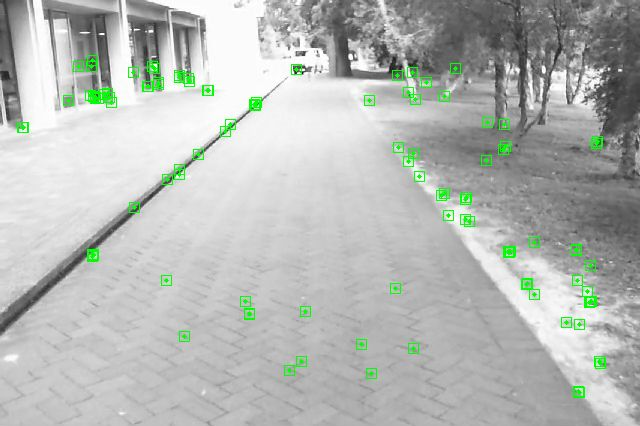
\includegraphics[width=0.8\linewidth]{fig10}
	\caption[Tracked ORB features]{ORB features tracked by ORB-SLAM2 as shown in bounding boxes.}
	\label{fig:4:orb1}
\end{figure}

\begin{figure}[H]
	\centering
	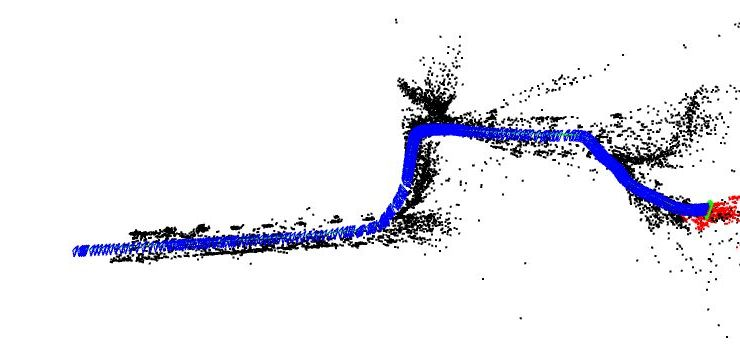
\includegraphics[width=0.8\linewidth]{fig11}
	\caption[ORB-SLAM2 trajectory]{Trajectory measured using ORB-SLAM2 for dead reckoning (blue), previously tracked ORB features (black) and presently tracked ORB features (red).}
	\label{fig:4:orb2}
\end{figure}

\section{Semantic Segmentation}\label{sec:4:semseg}
The incorporation of semantic segmentation into the MRS enables navigation to be supplemented with scene understanding and object classification. Semantic segmentation is a deep learning process that classifies each pixel in an image frame according to the object class it belongs to. This is especially useful in complex environments with multiple objects, with little uniformity in pose, features, and illumination.

\subsection{Semantic Segmentation Method}
For the semantic segmentation application of the MRS, SegNet~\cite{badrinarayanan_segnet:_2017} was selected based on its high compatibility and ease of implementation. The architecture of SegNet uses a convolution encoder and decoder setup that classifies objects from one of the following classes: sky, building, column-pole, road-marking, road, pavement, tree, sign-symbol, fence, vehicle, pedestrian and bicyclist; with a class average classification accuracy of 65.9\%~\cite{badrinarayanan_segnet:_2017}. This MRS uses SegNet whereby pedestrians, vehicles, buildings, vegetation, and pathways are classified as illustrated in Fig.~\ref{fig:4:ss1}, and are subsequently classified into static and dynamic objects.

Static objects are stationary (with stationary positions), while dynamic objects are moving (with time varying positions). It is important for an MR-SLAM system to differentiate static and dynamic objects to devise proper navigational reactions to the environment. For example, static objects such as buildings and vegetation are permanent placements in the environment; these objects will be mapped by the MR-SLAM algorithm as part of the environment. Conversely, dynamic objects such as pedestrians and vehicles are in motion or are temporary placements in the environment; these will not be mapped by the MR-SLAM algorithm. Overall, this process of differentiating object types will ultimately result in higher mapping accuracy, especially when the ground truth does not contain dynamic objects.

The recognition of dynamic objects also enables the system to estimate the motion of a specific moving object. In other words, by segregating moving vehicles or pedestrians within an image frame, the LiDAR can then be utilised to estimate the motion and trajectory of the said object. This enables the robot to actively perform obstacle avoidance according to its motion, which can be implemented by comparing the robot’s current speed against the LiDAR measurements on the classified dynamic object based on the image frame.

\subsection{Semantic Segmentation Evaluation}
Like visual odometry, semantic segmentation was also implemented in a decentralised approach onto individual UGVs. A Caffe~\cite{jia_caffe:_2014} implementation of SegNet is installed onto the individual UGVs, which enables pixelwise object classification that corresponds to LiDAR measurements at that time instance, which can be any of 12 classifiable classes. We subsequently separate these classes into static and dynamic classes. For example, bicycles, pedestrians, and vehicles are dynamic, whereas buildings, fences, pavement, poles, road, road markings, road signs, vegetation, and sky are static. By matching the position of the classified pixel at the $x$-axis against that of the LiDAR on a fixed $y$-plane, dynamic objects can therefore be segregated and tracked using the LiDAR for motion detection. Objects in motion will be compared against the trajectory of the UGV to ensure that there is no impending collision. These dynamic objects will also be ignored as part of the SLAM routine so that it does not become mapped as part of the environment.

\begin{figure}[H]
	\centering
	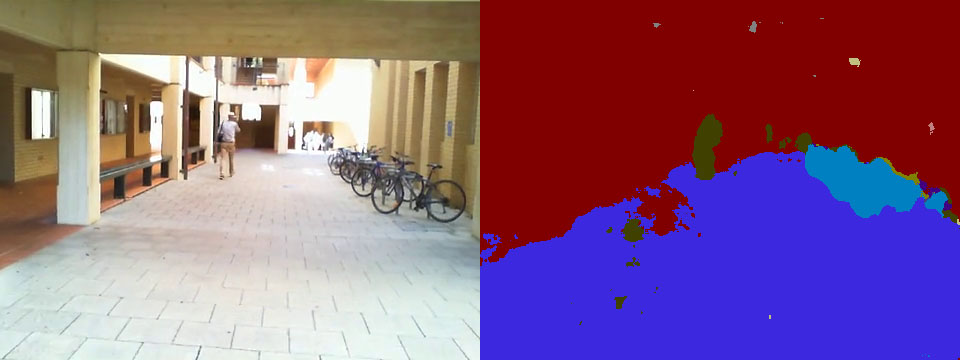
\includegraphics[width=0.8\linewidth]{fig12}
	\caption[SegNet output 1]{SegNet output showing segmented pedestrian (olive), bicycles (light blue), pathway (blue) and building (red).}
	\label{fig:4:ss1}
\end{figure}

Fig.~\ref{fig:4:ss1} was captured while navigating along the path as described in Section~\ref{sec:4:voe}. The parked bicycles on the right side and the pedestrians in the distance were properly segmented as dynamic objects, and the building and pavement as static objects. Several false detections are present due to variations in lighting and image quality, which accounts for 2.83\% of the total pixels classified on the pavement region.

\begin{figure}[H]
	\centering
	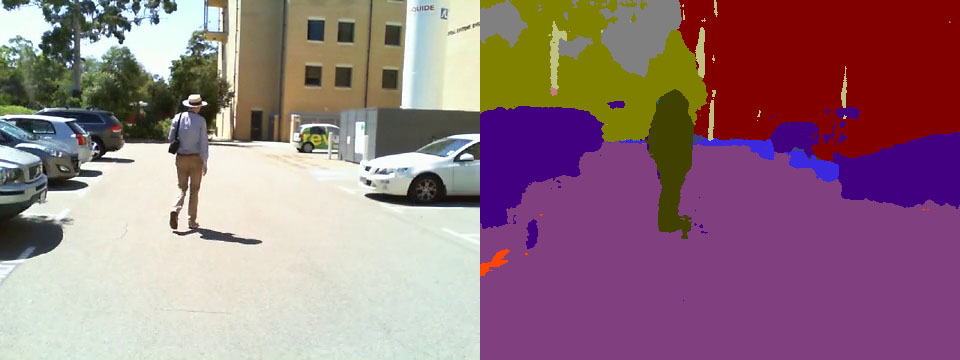
\includegraphics[width=0.8\linewidth]{fig13}
	\caption[SegNet output 2]{SegNet output from a parking area showing segmented road regions (purple), road markings (orange), and poles (yellow).}
	\label{fig:4:ss2}
\end{figure}

Fig.~\ref{fig:4:ss2} was also captured on the same path. While driving on roads, the road region and markings are properly classified along with the electric poles, vehicles, and pedestrians. Uniform lighting resulted in accurate classification accuracy with 0.69\% of all pixels falsely classified.

\section{Conclusion}
In this chapter, we have presented a decentralised multi-robot system for SLAM in urban outdoor environments together with visual odometry and semantic segmentation techniques. The vision-based methods can be used as an alternative to LiDAR-based localisation and object classification and may lead an overall cheaper and more powerful environmental perception system. We have presented an on-line, distributed, and decentralised MR-SLAM system that has proven to be resilient against environmental dynamics such as variations in lighting, terrain, pose, and moving objects. Evaluation results have confirmed the feasibility of using visual odometry as a viable solution to the odometry problem in an MRS, while semantic segmentation is a robust solution to object classification and scene understanding. Practical applications of this system can include search-and-rescue or reconnaissance missions in uncharted or hazardous environments, where detailed maps can be built quickly and accurately using a swarm of robots that are easily deployable, while being robust enough to cater to changes in the environment and hardware setup.